% !TeX spellcheck = en
\chapter{Implementation and experiments}
\label{sec:imp}

Here some code for my super neural network. 
The artificial neural networks discussed in this text are only remotely related to their biological counterparts. In this section we will briefly describe those characteristics of brain function that have inspired the development of artificial neural networks.

 
\begin{lstlisting}[caption={StudentFactory},captionpos=b]
class StudentFactory(DjangoModelFactory):
	class Meta:
		model = Student
	student_card = factory.SubFactory(StudentCardFactory)
	first_name = factory.Faker('first_name')
	second_name = factory.Faker('last_name')
\end{lstlisting}

\begin{wrapfigure}{l}{0.55\textwidth}
	\fbox{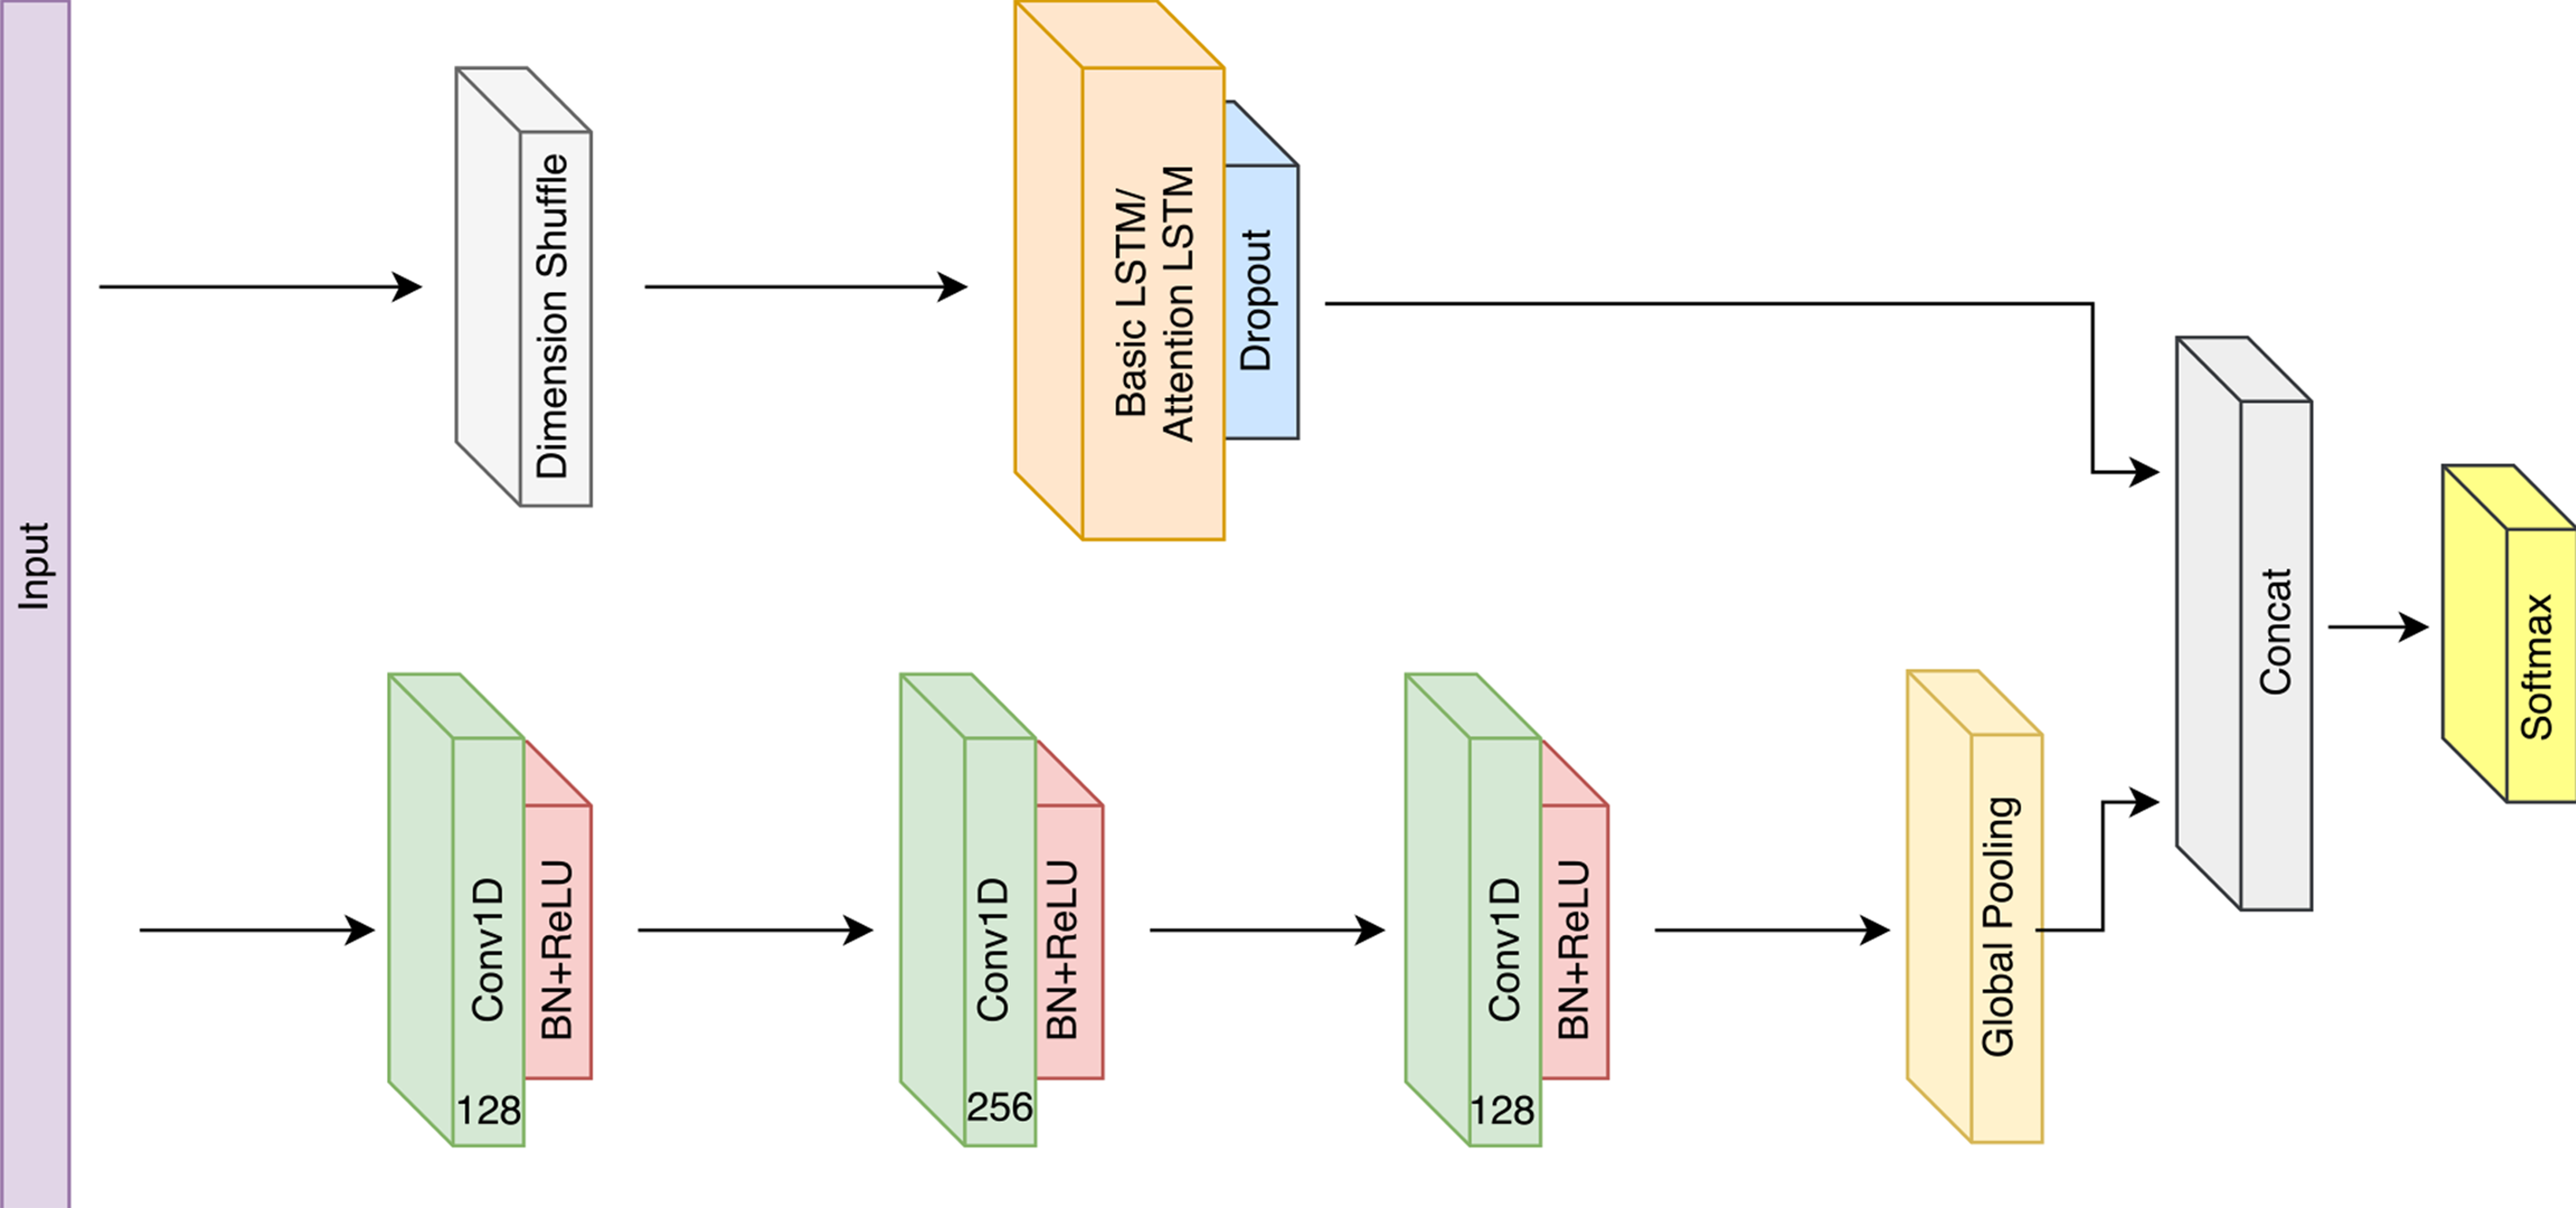
\includegraphics[width=0.5\textwidth]{gfx/LSTM-FCN.png}}
	\caption{LSTM Fully Convolutional Networks for Time Series Classification}
	\label{fig:nn1}
\end{wrapfigure}

You might already know that you want to apply an established theory or set of theories to a specific context (for example, reading a literary text through the lens of critical race theory, or using social impact theory in a market research project). 

\section{Implementation}
\label{sec:imp:programming}

\subsection{Unity application}
\label{sec:imp:programming:unity}
An application was developed in Unity with the Mixed Reality Toolkit and deployed on HoloLens 2. The goal of the application is to obtain the user position and orientation during the time a user wears a HMD. As this research aims to find an approach to reduce the M2P latency during rendering and delivering the volumetric content to end-user device, the volumetric animated object was placed three meters ahead of the user in Unity application. Users wearing HMD thus were asked to look on animated volumetric object and to move freely inside the laboratory space.\\
In Unity, the Main Camera is always the primary stereo rendering component attached to HMD and it is rendering everything the user sees \footnote{https://docs.microsoft.com/en-us/windows/mixed-reality/develop/unity/camera-in-unity}. The starting position of the user is set to $(0, 0, 0)$ during the application launch and the Main Camera tracks movement of the user's head. Although HoloLens allows to build a world-scale application, the room-scale experience was selected for spatial coordinate system. This lets users to walk around within the 5-meter boundary what is quite enough for user's movements inside the laboratory space and simultaneously watching the volumetric video object. 

\subsection{LSTM Model}
\label{sec:imp:programming:model}

\section{Experiments}
\label{sec:imp:experiments}
flipped quaternions

\subsection{Batch size}
A high impact on the performance e.g. the prediction accuracy has a batch size used in LSTM or GRU Model. The batch-size helps to learn the common patterns as important features by providing a fixed number of samples at one time. So that the model thus can distinguish the common features by looking at all the introduced samples of the batch. In most cases, an optimal batch size is set to 64. When this batch size was initially used with LSTM model, it gave significant high MSE, RMSE, train and validation errors. Based on the performance observation during experiments with LSTM parameters, batch size fine-tuning was done. The experiments done by \textit{Aykut et al} in their works \cite{delay_compensation_360} and \cite{telepresence} proved that appropriate batch size can be found in range $2^{9}$ - $2^{11}$ (512 - 2048). Notice that a power of 2 is used as a batch size. The overall idea is to fit a batch of samples entirely in the the CPU/GPU. Since, all the CPU/GPU comes with a storage capacity in power of two, it is advised to keep a batch size a power of two. Using a number different from a power of 2 could lead to poor performance.




\section{Evaluation metrics}
\label{sec:imp:eval}


\begin{figure}
	\centering
	\fbox{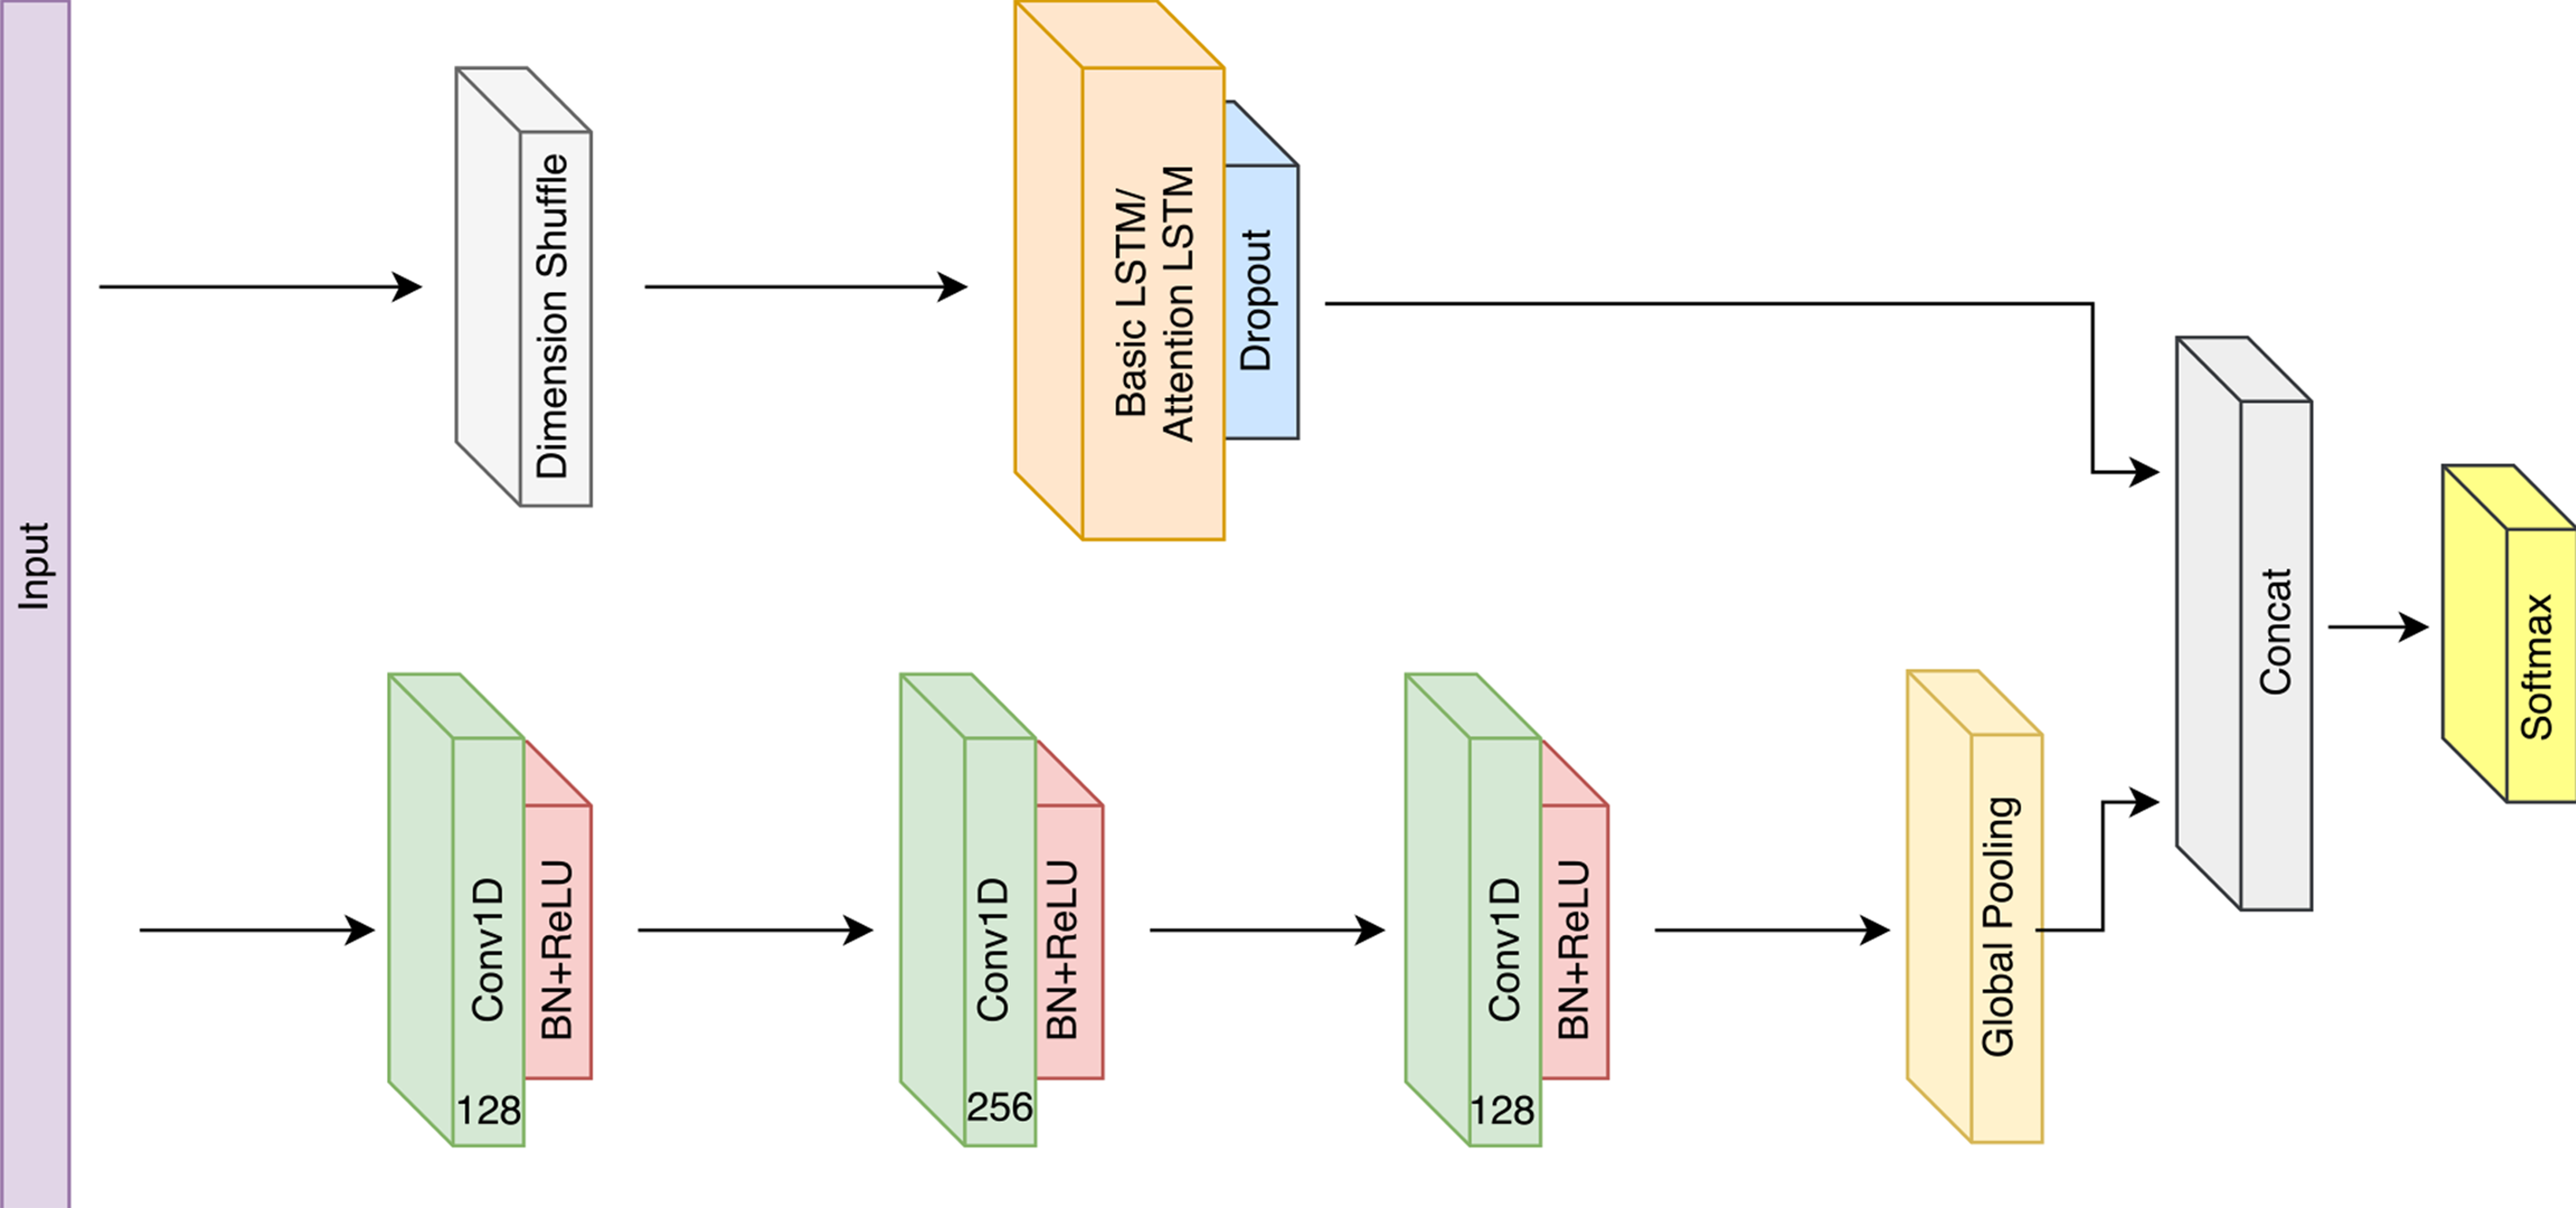
\includegraphics[width=1\textwidth]{gfx/LSTM-FCN.png}}
	\caption{LSTM FCN WRAP}
	\label{fig:nn2}
\end{figure}


\section{Results}
\label{sec:imp:results}
